\subsection{Chokepoints}
\label{sec:anfang_2}
Die Pfosten können jetzt mit Hilfe des Winkel- und Orientierungstest in rechte und linke Pfosten eingeteilt werden. Somit kann zwar ein Kanalpolygon erstellt werden, das allein reicht aber nicht für die Lösung. Das Kanalpolygon wird von allen Pfosten unterschiedlich stark eingegrenzt. Dabei existieren einzelne Pfosten, die das Kanalpolygon besonders stark einschränken. Diese kritischen Pfosten werden als \emph{Chokepoints} bezeichnet. Sie sind für das Berechnen der Schussgerade unabdingbar.\\

Die folgenden Abbildungen (\hyperref[fig:choke_equal]{Abb. 7} und \hyperref[fig:choke_diff]{Abb. 8}) verdeutlichen, dass die herkömmliche x- und y-Achsen-Aufteilung nicht ausreicht, um Chokepoints eindeutig zu bestimmen – es bedarf eines normierten Koordinatensystems (z.~B. basierend auf Isoklinen), um die relevanten Anteile der Höhe zwischen \(t_0\) und \(t_n\) zu erfassen.

\begin{figure}[h]
\centering
\label{fig:choke_equal}
    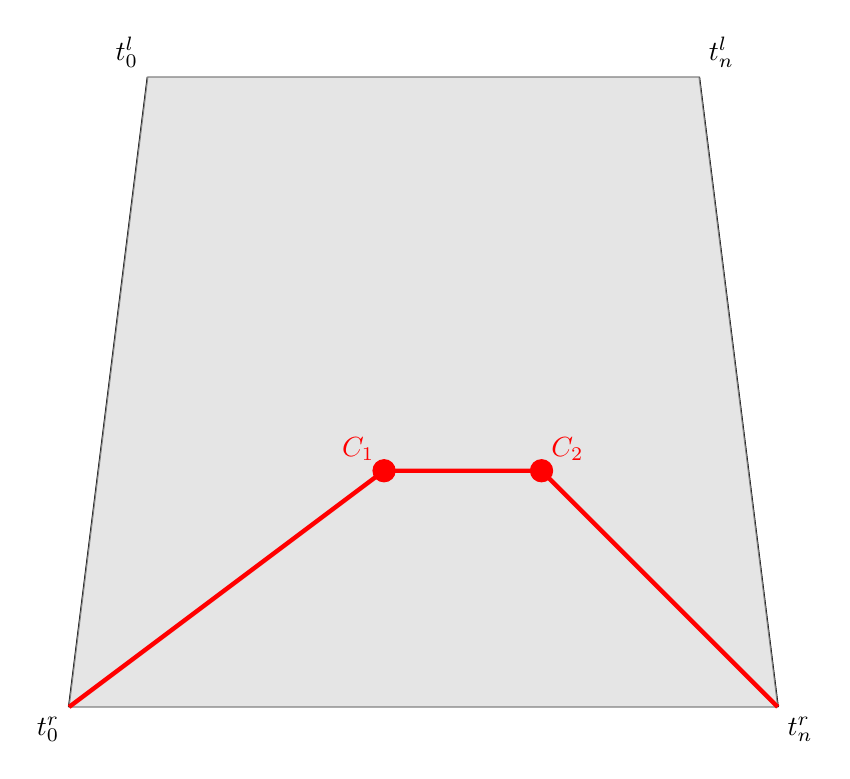
\begin{tikzpicture}[scale=2]

        \coordinate (t0R) at (0,0);
        \coordinate (t0L) at (0.5, 4);
        \coordinate (tnR) at (4.5, 0);
        \coordinate (tnL) at (4,4);

        \draw[thick] (t0L) -- (t0R);
        \draw[thick] (tnL) -- (tnR);
        \node[above left] at (t0L) {\(t_0^{l}\)};
        \node[below left] at (t0R) {\(t_0^{r}\)};
        \node[above right] at (tnL) {\(t_n^{l}\)};
        \node[below right] at (tnR) {\(t_n^{r}\)};

        \draw[gray, fill=gray!20] (t0L) -- (t0R) -- (tnR) -- (tnL) -- cycle;

        \coordinate (Cleft) at (2, 1.5);

        \coordinate (Cright) at (3,1.5);

        \draw[ultra thick, red] (t0R) -- (Cleft) -- (Cright) -- (tnR);
        \filldraw[red] (Cleft) circle (2pt) node[above left] {\(C_1\)};
        \filldraw[red] (Cright) circle (2pt) node[above right] {\(C_2\)};
        
    \end{tikzpicture}
    
	\caption{Chokepoints mit gleichem Einfluss auf das Kanalpolygon. Darstellung von zwei Chokepoints mit gleichem y-Wert \(C_1\) und \(C_2\), außerdem sind zwei Tore \(t_0\) und \(t_n\) abgebildet. Die schwarzen Linien sind das Initialpolygon und die roten Linien sind das Kanalpolygon. Beide Chokepoints schränken das Kanalpolygon ungefähr gleich stark ein.}
\end{figure}

\vspace{5cm}

\begin{figure}[h]
\centering
\label{fig:choke_diff}
	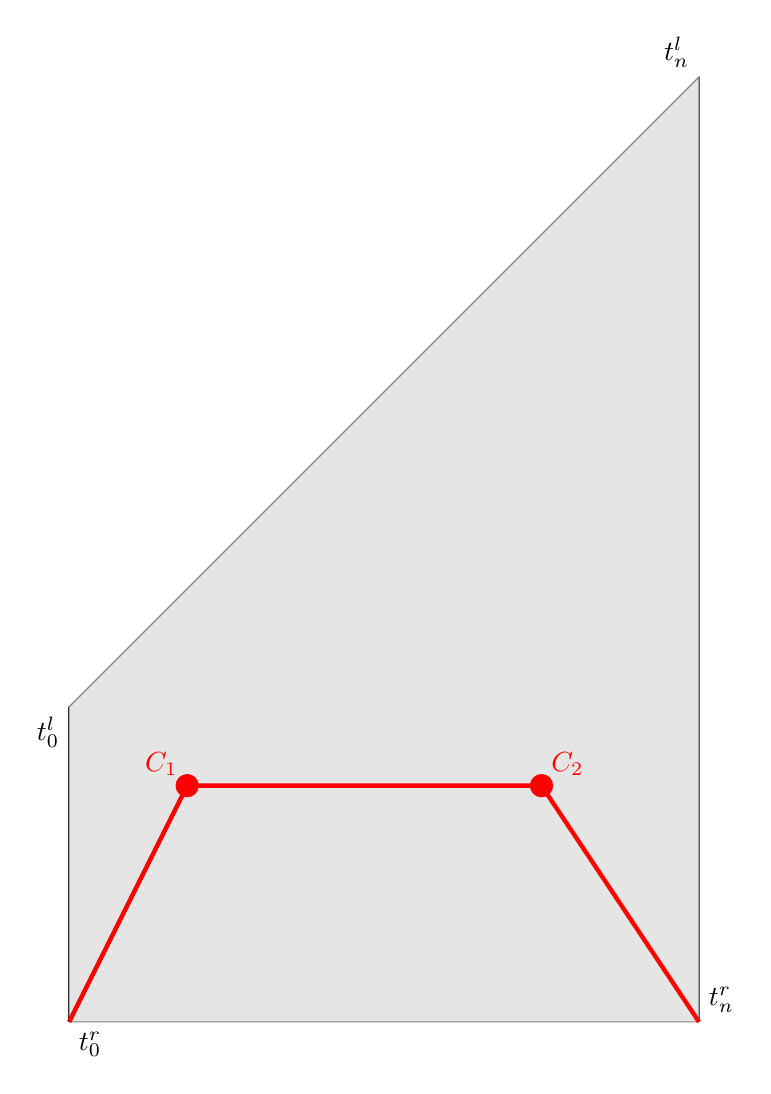
\begin{tikzpicture}[scale=2]

	\coordinate (t0R) at (0,0);
	\coordinate (t0L) at (0, 2);
	\coordinate (tnR) at (4, 0);
	\coordinate (tnL) at (4,6);
	
	\draw[thick] (t0L) -- (t0R);
	\draw[thick] (tnL) -- (tnR);
	\node[below left] at (t0L) {\(t_0^{l}\)};
	\node[below right] at (t0R) {\(t_0^{r}\)};
	\node[above left] at (tnL) {\(t_n^{l}\)};
	\node[above right] at (tnR) {\(t_n^{r}\)};
	
	\draw[gray, fill=gray!20] (t0L) -- (t0R) -- (tnR) -- (tnL) -- cycle;
	

	\coordinate (Cleft) at (0.75, 1.5);

	\coordinate (Cright) at (3,1.5);
	
	\draw[ultra thick, red] (t0R) -- (Cleft) -- (Cright) -- (tnR);
	\filldraw[red] (Cleft) circle (2pt) node[above left] {\(C_1\)};
	\filldraw[red] (Cright) circle (2pt) node[above right] {\(C_2\)};

	\end{tikzpicture}

    \caption{Chokepoints mit unterschiedlichem Einfluss auf das Kanalpolygon. Darstellung von zwei Chokepoints mit gleichem y-Wert \(C_1\) und \(C_2\), außerdem sind zwei Tore \(t_0\) und \(t_n\) abgebildet, \(t_0\) ist wesentlich kleiner als \(t_n\). Die schwarzen Linien stellen das Initialpolygon und die roten Linien  das Kanalpolygon dar. \(C_1\) schränkt das Kanalpolygon deutlich stärker ein als \(C_2\), obwohl beide im Koordinatensystem auf gleicher y-Höhe liegen.}
\end{figure}

\vspace{1em}

Aus den Beispielen lässt sich ableiten, dass die klassischen x- und y-Werte nicht sinnvoll zur Ermittlung von Chokepoints sind. Auch die Betrachtung von \(t_0\) und \(t_n\) als y-Achse bzw. \(ll\) und \(rr\) als x-Achse erweist sich als unzureichend, da diese Linien weder parallel zur x-/y-Achse noch untereinander parallel verlaufen müssen.

\newpage
\subsubsection{Verzerrte Ebene und Isoklinen}
\label{sec:ebene}
Um die im letzten Kapitel beschriebene Problematik zu überwinden, wird eine verzerrte Ebene eingeführt. Innerhalb eines beliebigen Vierecks kann so ein normiertes Koordinatensystem konstruiert werden, das die Pfosten relativ zueinander vermisst. Hierbei kommen Linien mit gleichen Abstandsproportionen zum Einsatz, die als \emph{Isoklinen} bezeichnet werden. Analog zu geographischen Koordinaten werden \emph{Längengrad-Isoklinen} (vergleichbar mit der x-Achse) und \emph{Breitengrad-Isoklinen} (vergleichbar mit der y-Achse) aufgebaut. Jeder Pfosten im initialen Viereck wird einer Steigung in Richtung des größeren Tores bzw. der längeren Linie (\(ll\) oder \(rr\)) zugeordnet.

Die Längengrad-Isoklinen geben an, wie nahe ein Pfosten an \(t_n\) liegt: Ein Pfosten auf \(t_0\) besitzt den Längengrad 0, während ein Pfosten auf \(t_n\) den Längengrad 1 aufweist. Die Breitengrad-Isoklinen bestimmen, wie nah ein Pfosten an \(rr\) liegt: Ein Breitengrad von 0 bedeutet, dass der Pfosten auf \(ll\) liegt, während ein Breitengrad von 1 anzeigt, dass der Pfosten auf \(rr\) liegt. So besitzt beispielsweise der linke Pfosten von \(t_0\) im normierten Koordinatensystem die Koordinaten \((0,0)\). Dies ermöglicht die Betrachtung des Problems im Einheitsquadrat – jeder Punkt ist eindeutig zuzuordnen. Ein Punkt, der 50\% des Wegs von \(t_0\) zu \(t_n\) zurückgelegt hat, liegt beispielsweise auf der 0,5-Längengrad-Isokline.

\subsubsection{Konstruktion von Längen- und Breitengrad-Isoklinen}
Für jeden Pfosten müssen die Längen- und Breitengrad-Isoklinen berechnet werden (\hyperref[fig:isoklinen]{Abb. 9}). Sind beispielsweise die Linien \(t_0\) und \(t_n\) parallel, verlaufen die Längengrad-Isoklinen ebenfalls parallel zu diesen Linien. In den meisten Fällen sind die Linienpaare jedoch nicht parallel, sodass deren charakteristische Funktionen einen gemeinsamen Schnittpunkt – den \emph{Ursprung} – besitzen. Dieser liegt außerhalb des Kanalpolygons. Für jeden Pfosten wird eine Isokline konstruiert, die den Pfosten mit diesem Urspung verbindet. Der Punkt, an dem die Isokline die kleinere der beiden Linien schneidet, dient zur Berechnung des relativen Abstands (Breite bzw. Länge) des Pfostens. Über diesen Ansatz können auch die Chokepoints identifiziert werden, die dem globalen Maximum der Breitengrad-Isoklinen entsprechen (sowohl für alle linken als auch für alle rechten Pfosten).


\begin{figure}[H]
\centering
\label{fig:isoklinen}
\begin{tikzpicture}[scale=1.5]

    \coordinate (A) at (1,1);
    \coordinate (B) at (0,3);
    \coordinate (C) at (4.5,5);
    \coordinate (D) at (3.5,-0.5);
    
    \draw[fill=gray!20, draw=black] (A) -- (B) -- (C) -- (D) -- cycle;
    
    \draw[thick, name path=t0] (A) -- (B) node[midway, left] {\(t_0\)};
    \draw[thick, name path=tn] (D) -- (C) node[midway, right] {\(t_n\)};
    
    \draw[blue, very thick, name path=ll] (A) -- (D) node[midway, below] {\(rr\)};
    \draw[blue, very thick, name path=rr] (B) -- (C) node[midway, above] {\(ll\)};
    
    \draw[dashed, gray] (A) -- ($ (B)!4!(A) $);
    \draw[dashed, gray] (D) -- ($ (C)!2!(D) $);
    \draw[dashed, gray] (A) -- ($ (D)!3!(A) $);
    \draw[dashed, gray] (B) -- ($ (C)!2!(B) $);
    
    \coordinate (A2) at (3.0333,-3.0667);
    \filldraw[red] (A2) circle (2pt) node[right] {\(U_2\)};
    
    \coordinate (A1) at (-1.34,2.41);
    \filldraw[green!70!black] (A1) circle (2pt) node[above] {\(U_1\)};
    

    \coordinate (P) at (2,2);
    \filldraw[black] (P) circle (2pt) node[above right] {\(P\)};
    
    \path[name path=Liso] (P) -- (A2);
    \draw[dashed, red] (P) -- (A2);
    
    \coordinate (S1) at (0.4,2.19);
    \filldraw[green!70!black] (S1) circle (2pt) node[above right] {\(S_1\)};
    \draw[dotted, green!70!black] (P) -- (S1);
    
    \path[name path=Biso] (P) -- (A1);
    \draw[dashed, green!70!black] (P) -- (A1);
    
    \coordinate (S2) at (2.35,0.2);
    \filldraw[red] (S2) circle (2pt) node[above right] {\(S_2\)};
    \draw[dotted, red] (P) -- (S2);
    
\end{tikzpicture}
\caption{Konstruktion von Längen- und Breitengrad-Isoklinen. Dargestellt sind zwei Linienpaare: die Tore \(t_0\), \(t_n\) und die Linien \(ll\) und \(rr\). Dort wo sich die erweiterten Linienpaare kreuzen, liegen die Urspünge \(U_1\) und \(U_2\). Von beiden Ursprüngen wird eine Linie, die jeweilige Isokline, zu dem Pfosten \(P\) gezogen. Die Schnittpunkte \(S_1\) und \(S_2\) der Isoklinen mit \(t_0\) bzw. \(rr\) sind markiert. Um die Isoklinenwerte zu berechnen wird die Lage des Schnittpunktes auf der jeweiligen Linie gemessen und als Wert zwischen 0 und 1 gespeichert.}
\end{figure}



\subsubsection{Filterung irrelevanter Pfosten}
\label{sec:ende_2}
Viele Pfosten im Kanalpolygon sind für die Bestimmung des gültigen Schusspfads irrelevant, da sie diesen nicht einschränken. Beim Berechnen der Isoklinen und bei der Suche nach Chokepoints können solche Pfosten herausgefiltert werden. Liegt der aktuelle Pfosten in Bezug auf den Längengrad niedriger als der vorherige, so befindet er sich näher an \(t_0\) – dies entspricht einer Bewegung „zurück“. Daraus entsteht ein Bereich im Kanalpolygon, der nicht Teil eines gültigen Schusspfads sein kann. Für das Herausfiltern solcher Bereiche sind die Steigungen der zwei letzten Streckensegmente des Kanalpolygons wichtig, einmal die Strecke von dem neuen Pfosten zu dem letzten (die neue Steigung) und die Strecke von dem letzten Pfosten zu dem vorletzten (die alte Steigung).

Um diese Situation zu differenzieren, werden folgende sechs Fälle betrachtet:
\begin{enumerate}
	\item Der neue Pfosten hat einen geringeren Breiten- und Längengrad als der vorherige Pfosten und die Steigungen haben unterschiedliche Vorzeichen.
	\begin{itemize}
		\item \textbf{Ergebnis:} Der vorherige Pfosten ist relevant, der neue ist irrelevant.
	\end{itemize}
	\item Der neue Pfosten hat einen geringeren Breiten- und Längengrad als der vorherige, die Steigungen haben gleiche Vorzeichen und die absolute neue Steigung ist größer als die absolute alte.
	\begin{itemize}
		\item \textbf{Ergebnis:} Der vorherige Pfosten ist relevant, der neue ist irrelevant.
	\end{itemize}
	\item Der neue Pfosten hat einen geringeren Breiten- und Längengrad als der vorherige, die Steigungen haben gleiche Vorzeichen und die absolute neue Steigung ist kleiner als die absolute alte.
	\begin{itemize}
		\item \textbf{Ergebnis:} Der vorherige Pfosten ist irrelevant, der neue ist relevant.
	\end{itemize}
	\item Der neue Pfosten hat einen geringeren Breitengrad, aber einen höheren Längengrad als der vorherige, und die Steigungen haben unterschiedliche Vorzeichen.
	\begin{itemize}
		\item \textbf{Ergebnis:} Der vorherige Pfosten ist irrelevant, der neue ist relevant.
	\end{itemize}
	\item Der neue Pfosten hat einen geringeren Breitengrad, aber einen höheren Längengrad als der vorherige, die Steigungen haben gleiche Vorzeichen und die absolute neue Steigung ist größer als die absolute alte.
	\begin{itemize}
		\item \textbf{Ergebnis:} Der vorherige Pfosten ist irrelevant, der neue ist relevant.
	\end{itemize}
	\item Der neue Pfosten hat einen geringeren Breitengrad, aber einen höheren Längengrad als der vorherige, die Steigungen haben gleiche Vorzeichen und die absolute neue Steigung ist kleiner als die absolute alte.
	\begin{itemize}
		\item \textbf{Ergebnis:} Der vorherige Pfosten ist relevant, der neue ist irrelevant.
	\end{itemize}
\end{enumerate}

So konnten bereits viele unwichtige Pfosten herausgefiltert werden. Übrig bleiben einzelne lokale Extremwerte (lokale Breitengrad-Minima), die entfernt werden können, um die Anzahl der Pfosten weiter zu reduzieren und so die Kanallinien zu glätten. Diese unwichtigen Pfosten muss der Algorithmus bei der Schusspfadberechnung nicht mehr beachten, wodurch der Algorithmus schneller wird. 
